\documentclass[11pt]{article}

\usepackage[margin=1in]{geometry}
\usepackage{amsmath,amssymb,amsthm}
\usepackage{bm}
\usepackage{hyperref}
\usepackage{tikz}
\usepackage{subcaption}
\usepackage{float}
\usetikzlibrary{positioning,fit,shapes.misc}
\setlength{\parindent}{0pt}
\setlength{\parskip}{0.7\baselineskip}

\title{Probabilistic Hierarchical Retention Time Prediction for LC--MS}
\author{Bioinformatics Team}
\date{\today}

\begin{document}

\maketitle

\section{Introduction}

This document describes a \textbf{probabilistic, multi-species, multi-compound hierarchical}
model to predict
LC--MS retention times for each (species, compound, run) combination, together with a
calibrated uncertainty. A simple baseline is to fit an independent supervised model
(for example, a lasso regression) for every species (or species group)--compound pair
using run-level features. In practice this ``one model per pair'' strategy fragments
the data, fails to share information across related species and compounds, behaves
poorly for rare or newly added combinations, and tends to overfit run covariates
instead of capturing global patterns of chromatographic drift.

We instead use a single hierarchical, multi-task regression model. Different
species and compounds are treated as related tasks that share information through
global priors: strongly supported effects can deviate from the average, while poorly
observed groups are shrunk gently toward a common pattern. This improves robustness in
small-data regimes and yields sensible behavior for rare or unseen combinations.

Two ingredients drive this sharing in the model family. First, each compound can be
represented by a \emph{descriptor}: a fixed-length numeric vector summarizing its
chemistry (for example, a PCA-compressed neural embedding or a fingerprint-derived
feature vector based on its SMILES string). Working in this shared descriptor space
lets the model generalize across chemically similar compounds and provide calibrated
priors for sparsely observed or new compounds. In the production configuration used
for the cap-based library runs and the primary figures in this document, we encode
chemistry directly via descriptors (for example, ChemBERTa PCA-20), and use discrete
chemical classes only to share run-covariate patterns.

Second, we include \emph{run covariates}: per-run features that summarize LC--MS
operating conditions. In the current system these covariates are derived from
internal-standard channels; endogenous standards and additional run-level signals can
be folded in the same way as they become available. These covariates allow the model
to explain systematic run-to-run shifts without training a separate model for every
run.

Taken together with the experiments in later sections, our current evidence suggests
that \textbf{a single hierarchical RT model, with chemistry encoded via descriptors
and classes used only to share run-sensitivity patterns, is the right direction for
generalisation across chemistry, rare compounds, and shifted runs}. The hierarchical
structure and descriptor-based chemistry encoding improve behaviour for rare species
and sparse chemistry, perform better than per-pair lasso in diverse species groups
such as cells, and show greater robustness to the kinds of run-level shifts we expect
when deploying kits and moving from Thermo-trained libraries to new instruments such
as Agilent. These capabilities are central to the RT work planned for 2026.

\section{Hierarchical Retention Time Model}

\subsection{Model specification}

At the observation level we work with simple $(s,c,r)$ indices:
\begin{itemize}
  \item $s$ = species (or species/matrix group),
  \item $c$ = compound,
  \item $r$ = LC--MS run,
  \item $y_{scr}$ = observed RT for species $s$, compound $c$, run $r$,
  \item $\bm{x}^{\star}_{r}\in\mathbb{R}^P$ = standardized run-covariate vector for run $r$
        (for example, internal-standard channels).
\end{itemize}

In these indices, the production configuration of the hierarchical RT model can be
written compactly as
\begin{align}
  y_{scr}
  &=
  \mu_0
  +
  \alpha_{s}
  +
  \beta_{c}
  +
  \bm{w}_{c}^{\top}\bm{x}^{\star}_{r}
  +
  \epsilon_{scr},
  &
  \epsilon_{scr} &\sim\mathcal{N}\!\bigl(0,\sigma^2_{y,k(s)}\bigr),
  \label{eq:rt-observation}\\[0.4em]
  \alpha_{s}
  &\sim\mathcal{N}\!\bigl(\mu^{\mathrm{(cluster)}}_{k(s)},\sigma^2_{\mathrm{species}}\bigr),
  &
  \mu^{\mathrm{(cluster)}}_{k}
  &\sim\mathcal{N}\!\bigl(0,\sigma^2_{\mathrm{cluster}}\bigr),
  \label{eq:rt-species}\\[0.4em]
  \beta_{c}
  &=
  \bm{z}_{c}^{\star\top}\bm{\theta}_\beta + \delta_c,
  &
  \delta_c &\sim \mathcal{N}\!\bigl(0,\sigma^2_{\mathrm{compound}}\bigr),
  \label{eq:rt-compound}
\end{align}
where $k(s)$ maps each species to a species cluster, $\bm{z}_c^{\star}\in\mathbb{R}^d$
is the standardized descriptor vector (for example, ChemBERTa PCA-20) for compound
$c$, and $\{\bm{w}_c\}$ are compound-specific covariate weights. In words:
$\mu_0$ is a global intercept (grand mean RT across species, compounds, and runs),
$\alpha_s$ is a species-level adjustment, $\beta_c$ is a descriptor-informed compound
baseline, and $\bm{w}_c^{\top}\bm{x}^{\star}_r$ captures how compound $c$ responds to
run-to-run shifts encoded by $\bm{x}^{\star}_r$.

The prior choices reflect weak information on a standardized scale and act as a form
of regularization. They keep group-level effects from becoming unrealistically large
in poorly observed settings, while still allowing the data to dominate when there is
ample evidence. In the current implementation we use HalfNormal priors on the key
scale parameters and Normal priors on fixed effects; these encourage shrinkage toward
zero without ruling out larger values when strongly supported by the data.

Variance components:
\begin{align}
  \sigma_{\mathrm{cluster}} &\sim \mathrm{HalfNormal}(0.5), \\
  \sigma_{\mathrm{species}} &\sim \mathrm{HalfNormal}(0.5), \\
  \sigma_{\mathrm{compound}} &\sim \mathrm{HalfNormal}(0.5).
\end{align}
The observation-noise scale is \emph{cluster-specific} in the production model:
for each species cluster $k$ we use
\begin{equation}
  \log \sigma_{y,k}\sim\mathcal{N}(\log 0.02,\,0.4^2),
  \qquad
  \sigma_{y,k} = \exp(\log \sigma_{y,k}),
\end{equation}
which corresponds to a log-normal prior centered near a typical within-cluster noise
scale (minutes) with moderate spread. For convenience in summaries we also define a
single scalar $\sigma_y$ as a root-mean-square aggregation over clusters.

For the global intercept and descriptor weights we use
\begin{equation}
  \mu_0\sim\mathcal{N}(\bar{t},5.0),
  \qquad
  \tau_\beta\sim\mathrm{HalfNormal}(0.6),
  \qquad
  \bm{\theta}_\beta\sim\mathcal{N}\bigl(\bm{0},\tau_\beta^2\,\bm{I}_d\bigr),
\end{equation}
where $\bar{t}$ is the empirical mean RT in the training data. This places a weakly
informative prior on the global intercept and on the descriptor-to-RT mapping.

For run-covariate weights, the implementation works with a compound-by-covariate
matrix $\gamma$ rather than an explicit $\bm{w}_c$. When covariates are present, we
use
\begin{equation}
  \sigma_\gamma\sim\mathrm{HalfNormal}(0.5),
  \qquad
  \gamma_{\text{raw}}[c,p]\sim\mathcal{N}(0,1),
\end{equation}
and set $\gamma[c,p]$ to a shrunk version of $\gamma_{\text{raw}}[c,p]$ around a
class-specific mean:
\begin{equation}
  \gamma_{\mathrm{class}}[\ell,p]\sim\mathcal{N}(0,\sigma^2_{\gamma,\mathrm{class}}),
  \qquad
  \gamma[c,p] = \gamma_{\mathrm{class}}\bigl(g(c),p\bigr)
                + \sigma_\gamma\,\gamma_{\text{raw}}[c,p].
\end{equation}
This encourages compounds in the same chemistry group to share covariate patterns,
while the half-normal priors on the relevant scales encourage small covariate
effects unless the data provide strong evidence for larger shifts.

The implementation uses non-centered parameterisations and sum-to-zero recentering
for the effects $\{\alpha_s\}$ and $\{\beta_c\}$ so that $\mu_0$ remains the grand
mean; these reparameterisations do not change the implied priors
in~\eqref{eq:rt-species}--\eqref{eq:rt-compound}. In the production configuration,
the covariate weights $\bm{w}_c$ follow the class-pooled hierarchy above, so that
compounds within the same chemical class share information about their run
sensitivities. Because the covariates are standardized (mean zero, unit variance per
component), the scale of the weights is interpretable and the model is numerically
well behaved.

\subsection{Lasso baseline and comparison}
\label{subsec:hier-structure}

\begin{figure}[H]
\centering
\begin{subfigure}[t]{0.45\textwidth}
\centering
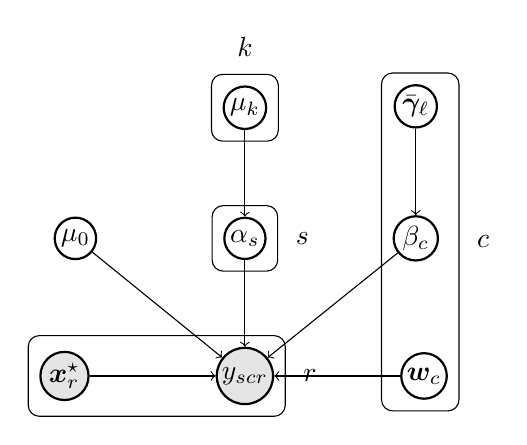
\begin{tikzpicture}[
  node distance=1.1cm,
  observed/.style={circle,draw,thick,inner sep=1pt,fill=gray!20},
  latent/.style={circle,draw,thick,inner sep=1pt},
  plate/.style={draw,rounded corners,inner sep=4pt}
]
  % Hierarchical RT model (tall schematic)
  \node[latent] (cluster) {$\mu_k$};
  \node[latent,below=1.1cm of cluster] (alpha) {$\alpha_s$};
  \node[observed,below=1.1cm of alpha] (y) {$y_{scr}$};
  \node[latent,left=1.6cm of alpha] (mu0) {$\mu_0$};
  \node[latent,right=1.6cm of alpha] (beta) {$\beta_c$};
  \node[latent,right=1.6cm of y] (w) {$\bm{w}_c$};
  \node[observed,left=1.6cm of y] (x) {$\bm{x}^{\star}_{r}$};
  \node[latent,above=1.1cm of beta] (class) {$\bar{\bm{\gamma}}_{\ell}$};

  \draw[->] (mu0) -- (y);
  \draw[->] (cluster) -- (alpha);
  \draw[->] (alpha) -- (y);
  \draw[->] (beta) -- (y);
  \draw[->] (w) -- (y);
  \draw[->] (class) -- (beta);
  \draw[->] (x) -- (y);

  \node[plate,fit=(cluster)] (plateK) {};
  \node at (plateK.north) [above=0.1cm] {$k$};

  \node[plate,fit=(alpha)] (plateS) {};
  \node at (plateS.east) [right=0.1cm] {$s$};

  \node[plate,fit=(beta) (w) (class)] (plateC) {};
  \node at (plateC.east) [right=0.1cm] {$c$};

  \node[plate,fit=(y) (x)] (plateR) {};
  \node at (plateR.east) [right=0.1cm] {$r$};
\end{tikzpicture}
\caption{Hierarchical RT model}
\label{fig:rt_hierarchical_plate}
\end{subfigure}
\hfill
\begin{subfigure}[t]{0.45\textwidth}
\centering
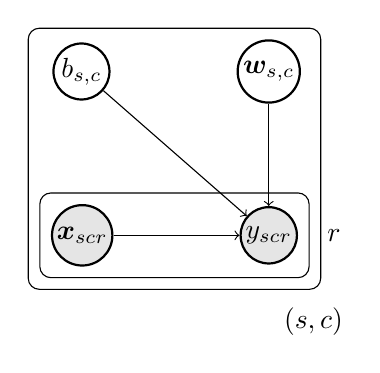
\begin{tikzpicture}[
  node distance=1.3cm,
  observed/.style={circle,draw,thick,inner sep=1pt,fill=gray!20},
  latent/.style={circle,draw,thick,inner sep=1pt},
  plate/.style={draw,rounded corners,inner sep=4pt}
]
  % Lasso baseline (tall schematic)
  \node[latent] (beta) {$\bm{w}_{s,c}$};
  \node[observed,below=1.3cm of beta] (y) {$y_{scr}$};
  \node[observed,left=1.6cm of y] (x) {$\bm{x}_{scr}$};
  \node[latent,left=1.6cm of beta] (b) {$b_{s,c}$};

  \draw[->] (b) -- (y);
  \draw[->] (beta) -- (y);
  \draw[->] (x) -- (y);

  \node[plate,fit=(y) (x)] (plateR) {};
  \node at (plateR.east) [right=0.1cm] {$r$};

  \node[plate,fit=(b) (beta) (plateR)] (plateGC) {};
  \node at (plateGC.south east) [below=0.1cm,xshift=-0.1cm] {$(s,c)$};
\end{tikzpicture}
\caption{Per-(group, compound) lasso}
\label{fig:rt_lasso_plate}
\end{subfigure}
\caption{Plate diagrams for the hierarchical RT model (left) and the per-(group, compound) lasso baseline (right). Shaded circles denote observed quantities (RT measurements $y_{scr}$ and run covariates $\bm{x}^{\star}_{r}$); unshaded circles denote latent variables and parameters. Indices: $s$ indexes species (or species/matrix groups), $c$ indexes compounds, $r$ indexes runs, $k$ indexes species clusters, and $\ell$ indexes chemical classes. In the hierarchical panel, $\mu_0$ is a global intercept, $\mu_k$ are cluster means, $\alpha_s$ are species effects, $\bar{\bm{\gamma}}_{\ell}$ are class-level mean run-covariate effects, $\beta_c$ are descriptor-informed compound baselines, and $\bm{w}_c$ are compound-specific covariate weights combining with run covariates $\bm{x}^{\star}_{r}$ to generate each observation $y_{scr}$. Plates labelled $k,s,c,r$ indicate replication over clusters, species, compounds, and runs. In the lasso panel, each $(s,c)$ has its own intercept $b_{s,c}$ and covariate weights $\bm{w}_{s,c}$ fitted independently, with the plate labelled $(s,c)$ denoting one separate regression per species--compound pair. For clarity, not all hyperparameters (such as the scale parameters $\sigma_\cdot$) or derived quantities are drawn; their roles are described in the surrounding text.}
\end{figure}

For comparison, the current lasso baseline used elsewhere in the pipeline fits a
separate penalised regression for each species (or matrix group) and compound. Fix a
species/matrix group $s$ and compound $c$, and let $r$ index runs with feature vectors
$\bm{x}^{\star}_{r}$ constructed from internal-standard and, when available,
endogenous-standard channels (columns such as ``IS*'', ``ES*'', and related
summaries). The lasso baseline fits an independent linear model
\begin{equation}
  y_{scr}
  =
  b_{s,c}
  +
  \bigl(\bm{x}^{\star}_{r}\bigr)^{\top}\bm{w}_{s,c}
  +
  \epsilon_{scr},
  \qquad
  \epsilon_{scr}\sim\mathcal{N}(0,\sigma_{s,c}^2),
\end{equation}
with parameters found by solving the penalised least-squares problem
\begin{equation}
  (\hat{b}_{s,c},\hat{\bm{w}}_{s,c})
  =
  \arg\min_{b,\bm{w}}
  \sum_{r}
    \bigl(y_{scr}-b-\bigl(\bm{x}^{\star}_{r}\bigr)^{\top}\bm{w}\bigr)^2
  +\lambda\lVert\bm{w}\rVert_1.
\end{equation}
Each $(s,c)$ pair is treated in isolation: there is no sharing of information across
groups, across compounds, or across related covariate patterns beyond the choice of
penalty $\lambda$.

The hierarchical RT model can be viewed as a structured generalisation of this
baseline. For the same species/matrix group $s$, compound $c$, and run $r$, it
uses the mean structure in~\eqref{eq:rt-observation} together with the
hierarchies in~\eqref{eq:rt-species}--\eqref{eq:rt-compound}. Informally, the
lasso parameters $b_{s,c}$ and $\bm{w}_{s,c}$ play a similar role to the
collapsed hierarchical intercept $\mu_0+\alpha_s+\beta_c$ and the
compound-specific weights $\bm{w}_c$, but without any sharing across groups or
compounds. Equivalently, we can view the hierarchical model as inducing
effective per-pair coefficients
\begin{equation}
  b^{(\mathrm{hier})}_{s,c}
  =
  \mu_0+\alpha_s+\beta_c,
  \qquad
  \bm{w}^{(\mathrm{hier})}_{s,c}
  =
  \bm{w}_c,
  \label{eq:hier-effective}
	\end{equation}
	so the hierarchical mean can be written in the same form as the lasso,
	but with $b^{(\mathrm{hier})}_{s,c}$ and $\bm{w}^{(\mathrm{hier})}_{s,c}$ tied
	across $(s,c)$ via shared priors on $\mu_0,\alpha_s,\beta_c$, and $\bm{w}_c$. This
	shared structure lets rare species--compound pairs borrow strength from well-sampled
	ones, while still behaving like per-pair regressions when data are abundant.

\subsection{Molecular descriptors (20-dim SMILES embedding)}

In the descriptor-augmented variant of the model we use per-compound molecular
descriptors $\bm{z}_c\in\mathbb{R}^{d}$ with a fixed
dimensionality $d=20$ to enable sharing across chemically similar compounds and to
provide calibrated priors for rarely observed or unseen compounds. Descriptors are
computed offline (for example, from a pretrained SMILES encoder or from fingerprint
features) and then passed into the model as a numeric matrix.

Before fitting we standardise each descriptor dimension across compounds to mean 0 and
variance 1. This internal standardisation keeps the prior on $\bm{\theta}_\beta$
well-scaled and ensures that no single descriptor coordinate dominates purely because
of its units. With centered descriptors, $\mu_0$ remains interpretable as the grand
mean RT. When descriptors are missing, we impute $\bm{z}_c$ to the zero vector in this
standardised space; in that case the model relies more heavily on the residual scale
$\sigma_{\mathrm{compound}}$ to represent uncertainty.

For typical library sizes, $d=20$ strikes a balance between expressiveness and sampling
stability. Larger descriptor dimensions increase cost and may require stronger
regularization without improving generalization, so in practice one can choose $d$
empirically and prefer the smallest value that matches held-out performance while
maintaining good sampler diagnostics.

\paragraph{Why this helps rare compounds.}
When descriptors are enabled, a rarely observed compound $c$ has its posterior
baseline $\beta_c$ shrink toward the descriptor-predicted mean
$\bm{z}_c^{\top}\bm{\theta}_\beta$ rather than a broad class average. Uncertainty
propagates both the mapping uncertainty in $\bm{\theta}_\beta$ and the residual scale
$\sigma_{\mathrm{compound}}$, yielding calibrated predictions.

\section{Inference, Uncertainty, and Diagnostics}

In practice we fit this model with the No-U-Turn Sampler (NUTS), using multiple chains
and standard adaptations of step size and tree depth. When a JAX/NumPyro backend is
available it can be used for faster gradient evaluations; otherwise the default PyMC
NUTS implementation is used. Typical runs involve a few hundred to a few thousand
posterior draws after warmup, with the exact configuration controlled by the sampling
arguments (\texttt{draws}, \texttt{tune}, \texttt{target\_accept}, and
\texttt{max\_treedepth}).

Given posterior draws, we summarise RT predictions for each species--compound pair
$(s,c)$ by reconstructing the linear predictor for a grid of runs and then computing
the predictive mean and variance. Writing $t_{sc}$ for the model's implied RT for
species $s$ and compound $c$, the implementation follows
\begin{equation}
  \hat{t}_{sc}=\mathbb{E}[t_{sc}],
  \qquad
  \hat{\sigma}^2_{sc}=\mathrm{Var}[t_{sc}]+\mathbb{E}[\sigma^2_{y,k(s)}],
\end{equation}
where the expectation and variance are taken over posterior draws. The first term
captures parameter uncertainty in the intercept, species, compounds, and covariate
weights, while the second term adds back the average observation-noise variance
$\sigma^2_{y,k(s)}$ to form a full predictive variance. At prediction time, helper routines
reconstruct the linear predictor for requested (species, compound, run) tuples using
posterior draws of $(\mu_0,\alpha_s,\beta_c,\bm{w}_c,\sigma_{y,k(s)})$ and return both mean
predictions and associated standard deviations $\hat{\sigma}_{sc}$.

Standard MCMC diagnostics (e.g.\ absence of divergences, $\hat{R}\le 1.01$,
$\mathrm{ESS}_{\mathrm{bulk}}\ge 200$) are enforced when assessing model fits. The
non-centered parameterisation and sum-to-zero recentering described in
Section~\ref{subsec:rt-noncentered} are chosen
precisely to make these diagnostics easier to satisfy in realistic LC--MS datasets.

Posterior predictive checks (PPC) are used to evaluate how well the model's predictive
distribution matches observed RTs. In the reference implementation we draw samples
from the posterior predictive distribution of $y_{\mathrm{obs}}$, compute per-row
predictive means, standard deviations, and central intervals (e.g.\ 95\%), and then
report summary metrics such as RMSE, MAE, empirical coverage of the 95\% interval, and
a small coverage curve at several nominal levels (0.5, 0.8, 0.9, 0.95). Simple residual
diagnostics (observed minus predictive mean) are also retained for downstream plots
and checks by species or chemistry group.

\section{Implementation details: data, training, and evaluation}

This section briefly describes how we construct the training datasets, fit the model,
and evaluate it against the existing lasso baseline. The aim is to clarify the
experimental setup rather than to spell out every engineering detail.

\subsection{Data preparation and capping}

For each library we start from a large merged RT dataset containing all labeled peaks,
with metadata for species, compound, matrix type, run identifiers, and internal
standards. We first restrict this dataset to rows with valid chemical classes and a
valid species mapping so that the downstream models work on a coherent set of
compounds and species.

We then apply a cap on the number of observations per species--compound--matrix
combination. If the cap is $N$, at most $N$ rows are retained for each such
combination, with rows selected at random using a fixed seed. This keeps the set of
species--compound pairs fixed while controlling how many replicate RT measurements
each pair contributes. Larger caps (for example, 20 or 50) therefore provide more
replicates per pair without changing which pairs are present.

After capping, we aggregate the internal-standard panels to form run-level covariates
and assemble an RT training table with one row per labeled peak. This table is the
input to the hierarchical model described in the earlier sections.

\subsection{Model training on capped datasets}

For each library and cap level we train a separate hierarchical RT model. The training
routine reads the capped RT table, constructs integer index spaces for species and
compounds, defines run indices from the run identifiers, and builds the standardized
run covariate vectors $\bm{x}^{\star}_r$ from the internal-standard measurements.

The hierarchical model is then fitted with NUTS using moderate chain and draw counts
chosen to balance runtime and diagnostics. Because the cap is enforced before
training, the model always sees the same structure (species, compounds, runs); only
the number of replicate observations per species--compound pair changes with the cap.

\subsection{Implementation details and non-centered parameterization}
\label{subsec:rt-noncentered}

This subsection is about sampler behaviour rather than modelling ideas; it is safe to
skip on a first read. Conceptually, the hierarchical model is fully described by the
centered priors in Section~\ref{subsec:hier-structure}, for example
\begin{equation}
  \alpha_{s}\sim\mathcal{N}\!\bigl(\mu_{k(s)},\sigma^2_{\mathrm{species}}\bigr),
  \qquad
  \beta_{c}\mid\mu_{g(c)}\sim
  \mathcal{N}\bigl(\mu_{g(c)},\ \sigma^2_{\mathrm{compound}}\bigr).
\end{equation}
Sampling these \emph{centered} group effects directly is intuitive but can lead to
``funnel''-shaped posteriors when the group-level scales (such as
$\sigma_{\mathrm{species}}$ or $\sigma_{\mathrm{compound}}$) are small. In those
regions, the sampler must explore very narrow, highly correlated directions, which can
cause slow mixing and divergent transitions for gradient-based methods like NUTS.

To avoid this we reparameterise the same model in a \emph{non-centered} form. Instead
of drawing $\alpha_s$ and $\beta_c$ directly, we draw standardised latent variables and
scale them by the corresponding standard deviations. For the cluster and species
effects we write
\begin{equation}
  \mu_k=\tilde{\mu}_k\,\sigma_{\mathrm{cluster}},
  \quad
  \tilde{\mu}_k\sim\mathcal{N}(0,1),
  \qquad
  \alpha_s=\mu_{k(s)}+\tilde{\alpha}_s\,\sigma_{\mathrm{species}},
  \quad
  \tilde{\alpha}_s\sim\mathcal{N}(0,1),
\end{equation}
and for the compound effects we use
\begin{equation}
  \tilde{\beta}_c\sim\mathcal{N}(0,1),
  \qquad
  \beta_c=\mu_{g(c)}+\tilde{\beta}_c\,\sigma_{\mathrm{compound}}.
\end{equation}

Mathematically this leaves the joint prior over $(\alpha_s,\beta_c)$ unchanged, but it
puts most of the curvature into the simple standard-normal variables
$(\tilde{\mu}_k,\tilde{\alpha}_s,\tilde{\beta}_c)$ and leaves the scale parameters
$(\sigma_{\mathrm{cluster}},\sigma_{\mathrm{species}},\sigma_{\mathrm{compound}})$ more
weakly correlated. In practice this geometry is much easier for NUTS to explore and
leads to fewer divergences.

As an additional implementation detail, we recenter the realised species effects so
that they have mean zero across species. This ``sum-to-zero'' adjustment keeps $\mu_0$
interpretable as the global RT level and helps separate overall shifts from
species-specific deviations, but it does not change the predictive distribution.

\subsection{Model implementation in \texttt{hierarchical.py}}

Equations~\eqref{eq:rt-observation} and~\eqref{eq:hier-effective} describe the
hierarchical RT model at the level of $(s,c,r)$ indices and effective per-pair
coefficients. The production implementation in
\texttt{src/compassign/rt/hierarchical.py} follows this specification closely, using
PyMC random variables for each component of the hierarchy and a non-centered
parameterisation for group effects.

\paragraph{Observation model \texorpdfstring{(\eqref{eq:rt-observation})}{(2.1)}.}
For convenience we restate the observation equation
\begin{align*}
  y_{scr}
  &=
  \mu_0
  +
  \alpha_{s}
  +
  \beta_{c}
  +
  \bm{w}_{c}^{\top}\bm{x}^{\star}_{r}
  +
  \epsilon_{scr},
  &
  \epsilon_{scr} &\sim\mathcal{N}\!\bigl(0,\sigma^2_{y,k(s)}\bigr),
\end{align*}
which the code implements directly. Inside \texttt{HierarchicalRTModel.build\_model},
the linear predictor corresponding to $y_{scr}$ is assembled as
\begin{verbatim}
rt_mean = (
    mu0
    + species_eff[species_idx]
    + compound_eff[compound_idx]
    + cov_term
    + sc_term
)
pm.Normal(
    "y_obs",
    mu=rt_mean,
    sigma=sigma_y_group[cluster_idx],
    observed=obs_df["rt"].values,
)
\end{verbatim}
Here \texttt{species\_idx}, \texttt{compound\_idx}, and \texttt{run\_idx} are the
integer indices for $(s,c,r)$, \texttt{mu0} implements $\mu_0$, \texttt{species\_eff}
implements $\alpha_s$, \texttt{compound\_eff} implements $\beta_c$, and \texttt{cov\_term}
implements $\bm{w}_c^{\top}\bm{x}^{\star}_r$. The term \texttt{sc\_term} is an optional
species--compound interaction intercept (enabled via \texttt{--species-compound-intercept}).
The vector \texttt{cluster\_idx} is derived from \texttt{species\_idx} via the species-to-cluster
mapping and selects the appropriate group noise scale $\sigma_{y,k(s)}$. The final line defines
$y_{scr}\sim\mathcal{N}(\texttt{rt\_mean},\sigma^2_{y,k(s)})$, matching the likelihood in
\eqref{eq:rt-observation}.

\paragraph{Group hierarchies.}
The species and cluster hierarchy in~\eqref{eq:rt-species} is implemented via
non-centered effects:
\begin{verbatim}
sigma_cluster = pm.HalfNormal("sigma_cluster", sigma=0.5)
sigma_species = pm.HalfNormal("sigma_species", sigma=0.5)
cluster_raw = pm.Normal("cluster_raw", 0.0, 1.0, shape=self.n_clusters)
cluster_eff = cluster_raw * sigma_cluster
cluster_eff = cluster_eff - pm.math.mean(cluster_eff)

species_raw = pm.Normal("species_raw", 0.0, 1.0, shape=self.n_species)
species_base = cluster_eff[self.species_cluster] + species_raw * sigma_species
species_eff = species_base - pm.math.mean(species_base)
\end{verbatim}
Drawing \texttt{cluster\_raw} and \texttt{species\_raw} from standard normals and
scaling by \texttt{sigma\_cluster} and \texttt{sigma\_species} gives the same
Gaussian priors as in~\eqref{eq:rt-species}, while subtracting the mean enforces the
sum-to-zero recentering described earlier. The compound baseline in
equation~\eqref{eq:rt-compound} is constructed as a descriptor term plus a compound residual,
\texttt{desc\_term + delta\_c}; when \texttt{include\_class\_hierarchy=True}, an additional
class-pooled component \texttt{class\_eff[self.compound\_class]} is added before recentering to
produce \texttt{compound\_eff}.

Run-covariate effects $\bm{w}_c$ are represented by the \texttt{gamma} tensor and
the standardised covariate matrix. For each observation the code computes
\texttt{cov\_term} as
\[
  \texttt{cov\_term}_i
  =
  \sum_{p}
    x^{\star}_{r(i),p}\,
    \gamma_{c(i),p},
\]
which is the dot product $\bm{w}_c^{\top}\bm{x}^{\star}_r$ in~\eqref{eq:rt-observation}
implemented as an elementwise product and sum over covariate dimensions.

\paragraph{Effective per-pair coefficients \texorpdfstring{(\eqref{eq:hier-effective})}{(2.4)}.}
The effective per-pair coefficients are given by
\begin{align*}
  b^{(\mathrm{hier})}_{s,c}
  &=
  \mu_0+\alpha_s+\beta_c,
  &
  \bm{w}^{(\mathrm{hier})}_{s,c}
  &=
  \bm{w}_c,
\end{align*}
and \texttt{HierarchicalRTModel.predict\_new} reconstructs these per-(species, compound)
coefficients from posterior draws:
\begin{verbatim}
mu0 = posterior["mu0"].values.flatten()
species_eff = posterior["species_eff"].values.reshape(-1, self.n_species)
compound_eff = posterior["compound_eff"].values.reshape(-1, self.n_compounds)
...
for i in range(n_samples_used):
    pred = (
        mu0[i]
        + species_eff[i, species_idx]
        + compound_eff[i, compound_idx]
    )
    if has_covariates:
        pred = pred + np.sum(cov_std * gamma[i][compound_idx], axis=1)
\end{verbatim}
For each posterior draw $i$, the term in parentheses plays the role of
$b^{(\mathrm{hier})}_{s,c}=\mu_0+\alpha_s+\beta_c$, and the row
\texttt{gamma[i][compound\_idx]} provides the per-compound covariate weights
$\bm{w}_c$ in~\eqref{eq:hier-effective}. The resulting predictions therefore have
exactly the hierarchical structure described in Section~2, but expressed as a
collection of coupled per-pair regressions in code.

\section{Results}

\subsection{Test set performance}

To assess out-of-sample performance we evaluate the hierarchical model on separate
real-test datasets that mirror the production schema but are held out from training.
For each library we reload the trained model and its posterior draws, align the
real-test species and compounds to the training index space, and compute predictive
means and uncertainties for all overlapping (species, compound, run) combinations.

In parallel we evaluate the existing per-pair lasso baseline on the same real-test
data. Each lasso model is a separate regression for a particular chemistry
supercategory and compound, with its own set of covariates and a prediction window.
During evaluation we only obtain lasso predictions for those compounds that have a
corresponding fitted model, so the lasso coverage can be substantially below one in
some species groups.

Figure~\ref{fig:rt_compare_lib208} summarises the comparison for one representative
setting: library 208, where the hierarchical model is trained on a cap-50 dataset and
evaluated on its real-test set alongside the lasso baseline. The top panel reports
RMSE in minutes by species group, and the bottom panel shows the fraction of
test-set compounds in each group for which each model produces a prediction. The
hierarchical model achieves lower RMSE than the lasso in most species groups, with
particularly clear gains for heterogeneous matrices such as fecal samples and human
cells, while the lasso is only marginally better in human blood and nearly tied in
urine. Across all groups the hierarchical model also maintains full compound coverage,
whereas the lasso typically leaves 10--25\% of compounds in each group without any
model.

\begin{figure}[H]
\centering

\includegraphics[width=\textwidth]{docs/models/images/rt_eval_compare_realtest_rmse_coverage_by_species_group_lib208_cap50.png}
\caption{Hierarchical RT model (blue) versus per-pair lasso baseline (orange) on the
lib208 real-test dataset when the hierarchical model is trained on a cap-50 RT
dataset. The upper panel shows RMSE by species group; the lower panel shows the
fraction of test-set compounds in each species group for which the model provides a
prediction (compound coverage).}
\label{fig:rt_compare_lib208}
\end{figure}

To give a sense of data usage, Table~\ref{tab:cap_rows} reports how many capped
training rows are used at different cap levels for libraries 208 and 209, and what
fraction of the full merged dataset they represent. The cap-50 configuration
underlying Figure~\ref{fig:rt_compare_lib208} uses only about 14\% of the available
labeled peaks in lib208 (and about 2\% in lib209) while keeping the full set of
species--compound pairs in each library.

\begin{table}[H]
\centering
\begin{tabular}{lrrrr}
\hline
Library & Cap & Training rows & Species--compound pairs & Rows as \% of full \\
\hline
208 & 5    & 80714   & 11054 & 1.58 \\
208 & 10   & 160782  & 11054 & 3.15 \\
208 & 20   & 315877  & 11054 & 6.20 \\
\textbf{208} & \textbf{50}   & \textbf{714672}  & \textbf{11054} & \textbf{14.02} \\
208 & 100  & 1185761 & 11054 & 23.26 \\
208 & 200  & 1792881 & 11054 & 35.17 \\
208 & 500  & 2764070 & 11054 & 54.22 \\
208 & 1000 & 3331202 & 11054 & 65.35 \\
209 & 5    & 258772  & 51364 & 0.26 \\
209 & 10   & 514122  & 51364 & 0.51 \\
209 & 20   & 998902  & 51364 & 0.99 \\
\textbf{209} & \textbf{50}   & \textbf{2187265} & \textbf{51364} & \textbf{2.17} \\
209 & 100  & 3452547 & 51364 & 3.43 \\
209 & 200  & 5202910 & 51364 & 5.16 \\
209 & 500  & 8750350 & 51364 & 8.68 \\
209 & 1000 & 12534514 & 51364 & 12.44 \\
\hline
\end{tabular}
\caption{Training set size for libraries 208 and 209 at different cap levels, taken
directly from the cap summary. Increasing the cap adds more replicate RT measurements
per species--compound pair without changing the set of pairs in each library.}
\label{tab:cap_rows}
\end{table}

Table~\ref{tab:rmse_by_group_lib208} shows RT RMSE and compound coverage by species
group for the same lib208 cap-50 experiment. On average across groups the hierarchical
model reduces RMSE from about 0.0166~min (lasso) to 0.0132~min, with the largest
relative gains in challenging matrices such as fecal samples and human cells. At the
same time the hierarchical model maintains essentially full compound coverage in all
groups, whereas the lasso baseline covers only around 76--90\% of compounds per
group.

\begin{table}[H]
\centering
\begin{tabular}{lcccc}
\hline
Species group & RMSE (hier) & RMSE (lasso) & Coverage (hier) & Coverage (lasso) \\
\hline
1 human blood              & 0.0136 & \textbf{0.0123} & 1.00 & 0.90 \\
2 mammal / rodent blood    & \textbf{0.0157} & 0.0215 & 1.00 & 0.89 \\
3 human / mammal fecal     & \textbf{0.0146} & 0.0217 & 1.00 & 0.86 \\
4 human / animal urine     & \textbf{0.0149} & 0.0156 & 1.00 & 0.82 \\
5 mammal tissue            & \textbf{0.0110} & 0.0129 & 1.00 & 0.78 \\
6 non-human cells + plants & \textbf{0.0099} & 0.0127 & 1.00 & 0.79 \\
8 human cells              & \textbf{0.0128} & 0.0196 & 1.00 & 0.76 \\
\hline
\end{tabular}
\caption{Per-species-group RMSE (minutes) and compound coverage for lib208, cap-50
training, evaluated on the real-test set. Coverage denotes the fraction of distinct
compounds in each species group for which the model produces a prediction.}
\label{tab:rmse_by_group_lib208}
\end{table}

One notable exception is human blood, where the per-pair lasso retains a small RMSE
advantage despite slightly lower coverage. This is consistent with the intuition that
in very well sampled, relatively homogeneous settings a separate linear model for each
species--compound pair is already close to optimal. In such regimes the hierarchical
model trades a small amount of best-case RMSE for a simpler shared structure. Natural
extensions to narrow this gap include adding a lightly regularised interaction term
for each species--compound pair (a hierarchical intercept $\delta_{s,c}$ that shrinks
to zero when data are sparse but allows per-pair flexibility when many observations
are available) and increasing the training cap specifically for high-data groups such
as human blood so that the hierarchy can better match the fine-grained structure that
lasso exploits there.

\subsection{Synthetic benchmarking of the RT hierarchy}

Beyond real-data evaluations, we benchmark the hierarchical RT model and its
descriptor-augmented variants on controlled synthetic datasets. These experiments are
designed to probe specific questions that are difficult to answer cleanly in
production data, such as how much descriptors help in sparse regimes, how well the
model extrapolates to unseen compounds and chemistry classes, and how robust it is to
covariate shift in run-level features.

\subsubsection{Descriptor ablation on synthetic RT}

The descriptor ablation experiment compares three arms of the hierarchical model on
synthetic RT data: a full model with descriptors and run covariates; a model with
descriptors but no covariates; and a model with covariates but no descriptors or
class hierarchy. Synthetic compounds are stratified into anchor, rare, and unseen
groups using the same descriptor space that feeds the model. Labels are allocated so
that anchors are moderately well observed, rare compounds have only a handful of
training labels, and unseen compounds are test-only.

For each replicate we fit all arms with matched sampler settings and report overall
and group-wise error metrics, together with MAE versus nearest-anchor distance. This
ablation isolates the contribution of descriptors over and above run covariates: in
our runs, \textbf{both descriptor-enabled arms achieve similar overall MAE and clearly
outperform the chemistry-free arm, with roughly 10--15\% MAE reduction for rare
compounds relative to the covariates-only arm}. For anchor compounds all three arms
are virtually indistinguishable. In this particular synthetic setup, adding
covariates on top of descriptors provides little extra gain, suggesting that chemistry
is doing most of the work and that run covariates mainly help align well-supported
compounds.

\begin{figure}[H]
\centering

\includegraphics[width=\textwidth]{docs/models/images/rt_desc_ablation_combined_tri_mae.png}
\caption{Descriptor ablation on synthetic RT. Mean MAE (with 95\% bootstrap intervals)
for three hierarchical arms---full (covariates + descriptors), descriptors without
covariates, and covariates without descriptors---shown overall and for rare
compounds. The descriptor-enabled arm achieves the lowest MAE for rare and unseen
compounds while matching the chemistry-free arm when support is high.}
\label{fig:rt_desc_ablation}
\end{figure}

\subsubsection{Generalisation to unseen compounds and classes}

A second set of experiments probes how descriptor-informed hierarchies generalise
across chemistry. We consider two synthetic scenarios. In a cold-start setting, a
subset of compounds is held out entirely from training and only evaluated at test
time, while anchors and rare compounds are used for fitting. This mirrors the
practical case where a new compound is added to a library: no labeled RTs for that
compound are available when the model is trained, but we still need a reasonable RT
prior based on descriptors and run covariates.

In a mix-shift setting, entire chemistry classes are held out from training and only
evaluated at test time, so that the model must extrapolate across descriptor space
rather than across runs. This corresponds to situations where the chemistry mix in a
study differs substantially from the mix in the training library—for example, when a
platform trained on mostly lipids is applied to a study enriched for steroids or
phospholipids. The question is whether the descriptor hierarchy can transfer what it
learns from well-sampled classes to structurally related but unobserved classes.

In both scenarios we compare the hierarchical RT model with and without descriptors,
using the same underlying synthetic generator and training splits. We evaluate MAE,
RMSE, bias, and tail error for unseen compounds and held-out classes versus their
seen counterparts. \textbf{Across replicates the descriptor-enabled hierarchy reduces
MAE for unseen compounds by roughly 30--40\% compared with the no-descriptor
hierarchy, with similar gains for held-out classes while leaving error on seen
chemistry essentially unchanged or slightly improved}. These synthetic results
support the view that the descriptor prior is genuinely enabling extrapolation across
chemistry rather than merely smoothing within well-sampled classes.

\begin{figure}[H]
\centering

\includegraphics[width=\textwidth]{docs/models/images/rt_desc_generalization_combined_mae.png}
\caption{Descriptor generalisation on synthetic RT. Mean MAE for the hierarchical
model with and without descriptors under two scenarios: unseen compounds (cold start)
and held-out chemistry classes (mix shift). Descriptors substantially reduce MAE for
truly unseen chemistry while leaving performance on seen compounds and classes
unchanged or slightly improved.}
\label{fig:rt_desc_generalization}
\end{figure}

\subsubsection{Descriptor robustness under run-level drift}

To study robustness under run-level covariate drift we generate synthetic datasets
with internal-standard covariates and descriptors, fix a set of in-support runs for
training, and evaluate several methods on held-out runs. We compare a hierarchical
model with descriptors, a chemistry-free hierarchical model, and two lasso baselines
that operate at the species--compound and cluster--compound levels. All methods are
evaluated twice on the same held-out rows: once using the original run covariates and
once after perturbing the covariates along an internal-standard-weighted drift
direction.

The resulting MAE and RMSE curves show how each method degrades as drift is applied.
\textbf{In our synthetic runs the descriptor-enabled hierarchy remains competitive
with the best lasso baseline under observed covariates and becomes clearly superior
once drift is applied: its MAE increases only slightly, whereas both the
chemistry-free hierarchy and the baselines show noticeably larger degradation}. This
suggests that descriptor-informed pooling helps stabilise predictions for runs that
move modestly out of the training covariate support, although it does not remove the
impact of large drifts.

\begin{figure}[H]
\centering

\includegraphics[width=\textwidth]{docs/models/images/rt_desc_shift_combined_mae.png}
\caption{Descriptor-informed hierarchy under synthetic run-level drift. Mean MAE for
hierarchical models with and without descriptors, and for species×compound and
cluster×compound lasso baselines, evaluated on the same held-out runs with observed
covariates and with induced drift. The descriptor-enabled hierarchy degrades more
slowly under drift than the chemistry-free hierarchy and lasso baselines.}
\label{fig:rt_desc_shift}
\end{figure}

\subsubsection{Covariate-shift holdout for historical baselines}

Finally, we revisit an earlier covariate-shift benchmark that predates the use of
descriptors. In this experiment we generate synthetic RT data with internal-standard
covariates, identify in-support runs using a global distance-to-nearest-neighbour
score in covariate space, and train the hierarchical RT model (without descriptors)
and lasso baselines on those in-support runs. Out-of-support runs are partitioned
into distance bins, and all methods are evaluated on each bin.

This study provides a baseline view of how the pre-descriptor hierarchy behaves under
progressive covariate shift. \textbf{Even without descriptors the hierarchical model
tends to degrade more gracefully than per-pair lasso fits as runs move further from
the training support, especially when a small number of anchors is available to
recalibrate intercepts, although all methods incur substantial error in the most
extreme out-of-support bins}. The descriptor-focused experiments above build on this
foundation to quantify how much additional robustness and generalisation we gain by
making the hierarchy explicitly chemistry-aware.

\begin{figure}[H]
\centering
\begin{subfigure}[t]{\textwidth}
\centering

\includegraphics[width=\textwidth]{docs/models/images/rt_covshift_holdout_mae_anchors0.png}
\caption{0 anchors}
\end{subfigure}

\vspace{0.5\baselineskip}

\begin{subfigure}[t]{\textwidth}
\centering

\includegraphics[width=\textwidth]{docs/models/images/rt_covshift_holdout_mae_anchors3.png}
\caption{3 anchors}
\end{subfigure}

\vspace{0.5\baselineskip}

\begin{subfigure}[t]{\textwidth}
\centering

\includegraphics[width=\textwidth]{docs/models/images/rt_covshift_holdout_mae_anchors5.png}
\caption{5 anchors}
\end{subfigure}
\caption{Covariate-shift holdout on synthetic RT. Each panel shows mean MAE (with
95\% intervals) for the hierarchical RT model and two lasso baselines across
increasing covariate-distance bins, for different numbers of anchor observations per
test run. Even without descriptors, the hierarchical model degrades more smoothly
under covariate shift than the lasso baselines, and a modest number of anchors
substantially improves calibration.}
\label{fig:rt_covshift_holdout}
\end{figure}

\section{Conclusions and future work}

We have described a hierarchical RT model for LC--MS that pools information across
species, compounds, and runs while retaining interpretable components such as species
effects, descriptor-informed compound baselines, and class-pooled run-level covariate
sensitivities. By replacing per-(species, compound) lasso fits
with a single multi-task hierarchy, the model provides a coherent framework for
borrowing strength across related tasks and for obtaining calibrated uncertainties.

On production-style data the hierarchical model (in its descriptor-based configuration
with class-pooled covariate effects) matches or improves upon the existing lasso baseline across most
species groups while maintaining nearly complete compound coverage. Synthetic
experiments show that descriptors are particularly valuable for rare and unseen
compounds and for held-out chemistry classes, and that the hierarchy degrades more
gracefully than lasso baselines under run-level covariate drift and covariate shift.
Together, these results indicate that the hierarchical RT model, with a chemistry
prior based on descriptors and classes used only to share run sensitivities, is a promising backbone for
future RT modelling in settings with sparse chemistry, diverse species groups, and
evolving instrumentation.

At the same time, several important pieces of work remain before this model can be
treated as a fully mature production component:

\begin{itemize}
  \item \textbf{Systematic convergence diagnostics for production fits.} The lib208
  results presented here are based on NUTS runs that were not exhaustively checked
  for convergence (e.g.\ detailed R-hat, ESS, and divergence inspection per group).
  We need a routine convergence review and alerting pipeline for all production
  fits, including stress tests on difficult species groups and chemistries.

  \item \textbf{Scalable inference on modern hardware.} Full NUTS on large libraries
  remains expensive. We should investigate GPU-backed samplers (for example via
  JAX/NumPyro) and carefully designed approximate methods such as variational
  inference or structured Laplace approximations. These approaches are non-trivial
  to deploy safely but could provide the order-of-magnitude speedups needed for
  routine retraining and cross-validation.

  \item \textbf{Principled propagation of RT uncertainty into peak assignment.}
  Downstream peak assignment currently relies on relatively ad hoc RT windows tuned
  for lasso. A key next step is to integrate RT predictive means and variances into
  the peak-assignment objective so that assignments are scored using the full
  predictive distribution rather than hard thresholds, and so that uncertainty is
  carried through to downstream confidence metrics.

  \item \textbf{Cross-instrument and cross-kit generalisation.} The experiments here
  focus on a single platform (Thermo-trained libraries). For 2026 we need to explore
  cross-instrument modelling---for example, hierarchical structures with instrument-
  level effects or shared descriptor priors---and assess how well RT predictions
  transfer to new instruments such as Agilent and to new kit designs with different
  chemistry and matrix mixes. Concrete options include instrument-specific offsets
  on the global intercept and descriptor weights, shared descriptor coefficients with
  partial pooling across instruments, and using anchor compounds measured on multiple
  platforms to identify and correct systematic cross-instrument shifts.

  \item \textbf{Model refinements in high-data regimes.} The hierarchical model
  slightly lags the lasso baseline in very well sampled, homogeneous groups such as
  human blood, where a separate linear model per species--compound pair is close to
  optimal. To narrow this gap without sacrificing behaviour in sparse settings, we
  can introduce a species--compound interaction term (a hierarchical intercept
  $\delta_{s,c}$ that shrinks toward zero when few observations are available but
  behaves like a per-pair correction when data are plentiful), experiment with
  descriptor-informed covariate slopes for run features in place of or in addition to
  the current class-pooled structure, and tune caps or priors on a per-group basis so
  that especially data-rich groups can make fuller use of their additional
  information.
\end{itemize}

Addressing these items will turn the current RT hierarchy from a promising component
into a robust foundation for kit deployment across rare species, diverse chemistries,
and new instruments.

\end{document}
